\documentclass[12pt]{article}
\usepackage{amsmath}
\usepackage{graphicx}
\usepackage{float}
\usepackage{caption}
\usepackage{subcaption}
\usepackage[margin=1in]{geometry}

\title{ELCT 562 CA2}
\author{J. Vaught}
\date{\today}

\begin{document}

\maketitle

\section{Introduction}
This document presents the analysis of a MATLAB simulation to generate and analyze a multipath channel response based on the Extended Pedestrian A (EPA) model. The simulation accounts for Rayleigh fading on each multipath component.

\section{The \texttt{pathGen} Function}
The MATLAB function \texttt{pathGen} is designed to generate random complex gains for a multipath channel, where each path follows Rayleigh fading. The power of the channel is normalized such that the sum of the squares of the path gains is 1. Here is the function definition:

\begin{verbatim}
function [pathComplexGainsRandom] = pathGen(relativePowersIndB)
    % Convert relative powers from dB to linear scale
    relativePowersLinear = 10.^(relativePowersIndB / 10);
    
    % Number of paths
    L = length(relativePowersLinear);

    % Generate random complex gains for each path
    % Assuming Rayleigh fading, each path amplitude follows a Rayleigh distribution
    % and each path phase is uniformly distributed between 0 and 2*pi
    pathAmplitudes = sqrt(relativePowersLinear) .* raylrnd(sqrt(2)/2, [1, L]);
    pathPhases = exp(1i * 2 * pi * rand(1, L));

    % Calculate complex path gains
    pathComplexGains = pathAmplitudes .* pathPhases;

    % Normalize the power of the channel
    normalizationFactor = sqrt(sum(abs(pathComplexGains).^2));
    pathComplexGainsRandom = pathComplexGains / normalizationFactor;
end
\end{verbatim}

\subsection{Function Mechanics}
The function operates as follows:

\begin{enumerate}
    \item Convert the input relative powers from dB to a linear scale using the equation:
    \[ \text{Power (linear)} = 10^{\frac{\text{Power (dB)}}{10}}. \]

    \item For each path, generate a complex gain to simulate Rayleigh fading. The amplitude of the gain is modeled as a Rayleigh distributed variable and the phase is uniformly distributed between 0 and \( 2\pi \). This is mathematically represented as:
    \[ h_i = X_i \cdot e^{j\theta_i}, \]
    where \( X_i \) is a Rayleigh distributed variable with parameter \( \sigma = \sqrt{\frac{\text{Power (linear)}}{2}} \) and \( \theta_i \) is a uniform random variable between 0 and \( 2\pi \).

    \item Normalize the path gains so that the channel's total power is 1, fulfilling the condition:
    \[ \sum_{i=1}^{L} |h_i|^2 = 1. \]
    The normalization is achieved by dividing each path gain by the square root of the sum of the squared magnitudes of all path gains:
    \[ h_i = \frac{h_i}{\sqrt{\sum_{i=1}^{L} |h_i|^2}}. \]
\end{enumerate}

\section{Main Code Analysis}
The main code is responsible for invoking the \texttt{pathGen} function to simulate the multipath channel response and for performing the statistical analysis of the results. The code is structured as follows:

\begin{itemize}
    \item \textbf{Initialization}: Define the relative power levels for the EPA profile and prepare variables for accumulating statistical data.
    
    \item \textbf{Simulation Loop}: Execute a loop to generate 10,000 independent channel realizations using \texttt{pathGen}.
    
    \item \textbf{Collection of Statistics}: Within the loop, calculate and accumulate the squared magnitudes of the path gains for each path and for the sum over all paths.
    
    \item \textbf{Post-Processing}: After completing all realizations, compute the mean of the squared magnitudes and the mean sum of the squared magnitudes to verify normalization.
    
    \item \textbf{Relative Power Calculation}: Calculate the relative powers in dB for each path to assess the attenuation of each multipath component compared to the first path.
    
    \item \textbf{Comparison with Theoretical Values}: Compare the simulation results with theoretical values to evaluate the accuracy of the simulation.
    
    \item \textbf{Plotting}: Visualize the mean squared magnitudes and relative powers using bar plots for an intuitive comparison with theoretical values.
\end{itemize}
\newline\newline
The MATLAB script for this analysis could be illustrated as:

\begin{verbatim}
clc;
clear
close all;

% Define the EPA model relative powers in dB
relativePowersEPA_dB = [0.0, -1.0, -2.0, -3.0, -8.0, -17.2, -20.8];
L = length(relativePowersEPA_dB); % Number of paths

% Initialize arrays to store the results
meanAbsH2 = zeros(1, L);
sumMeanAbsH2 = 0;

% Perform the analysis for 10000 realizations
numRealizations = 10000;
for n = 1:numRealizations
    pathGains = pathGen(relativePowersEPA_dB);
    meanAbsH2 = meanAbsH2 + abs(pathGains).^2;
    sumMeanAbsH2 = sumMeanAbsH2 + sum(abs(pathGains).^2);
end
meanAbsH2 = meanAbsH2 / numRealizations;
sumMeanAbsH2 = sumMeanAbsH2 / numRealizations;

% a. Tabulate mean of |h_i|^2 for i = 1,2, ..., L
disp('Mean of |h_i|^2 for each path:');
disp(meanAbsH2);

% b. Mean of the sum of |h_i|^2
disp('Mean of the sum of |h_i|^2 over all paths:');
disp(sumMeanAbsH2);

% c. Calculate and tabulate 10log10 of the mean of |h_i|^2
relativePowerdB = 10 * log10(meanAbsH2 / meanAbsH2(1));
disp('Relative power in dB compared to the first path:');
disp(relativePowerdB);

% Compare with theoretical values
disp('Theoretical Relative Powers in dB (EPA Model):');
disp(relativePowersEPA_dB);

% a. Mean of |h_i|^2 for each path
figure;
bar(1:L, meanAbsH2);
title('Mean of |h_i|^2 for Each Path');
xlabel('Path Index (i)');
ylabel('Mean of |h_i|^2');
grid on;

% Theoretical values of |h_i|^2 (linear scale)
theoreticalPowersLinear = 10.^(relativePowersEPA_dB / 10);
theoreticalPowersLinear = theoreticalPowersLinear / sum(theoreticalPowersLinear);
hold on;
plot(1:L, theoreticalPowersLinear, 'r*-');
legend('Calculated', 'Theoretical');
hold off;

% c. Relative power in dB compared to the first path
figure;
bar(1:L, relativePowerdB);
title('Relative Power in dB Compared to the First Path');
xlabel('Path Index (i)');
ylabel('Relative Power (dB)');
grid on;

% Plot theoretical values for comparison
hold on;
plot(1:L, relativePowersEPA_dB - relativePowersEPA_dB(1), 'r*-');
legend('Calculated', 'Theoretical');
hold off;


\end{verbatim}
\clearpage
\section{Results and Discussion}
The analysis yielded the following results:

\begin{itemize}
    \item Mean of \( |h_i|^2 \) for each path: \\
    0.3000, 0.2519, 0.2075, 0.1686, 0.0608, 0.0079, 0.0034
    \item Mean of the sum of \( |h_i|^2 \) over all paths: \\
    1
    \item Relative power in dB compared to the first path: \\
    0, -0.7592, -1.5997, -2.5014, -6.9334, -15.7971, -19.5190
\end{itemize}

Theoretical relative powers for the EPA model were provided for comparison. The calculated mean powers are close to the theoretical values, with small discrepancies likely due to the finite number of realizations and random variations inherent to Rayleigh fading.

\subsection{Mean of \( |h_i|^2 \) for Each Path}
\begin{figure}[H]
\centering
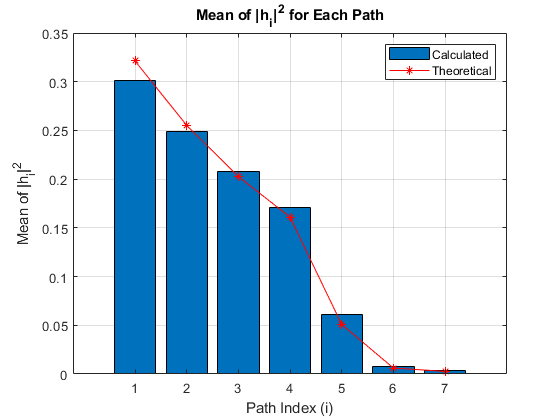
\includegraphics[width=0.7\textwidth]{path1.png}
\caption{Mean of \( |h_i|^2 \) for each path.}
\end{figure}

\subsection{Relative Power in dB}
\begin{figure}[H]
\centering
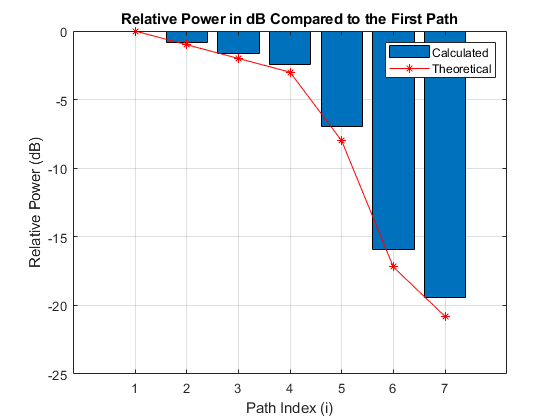
\includegraphics[width=0.7\textwidth]{path2.png}
\caption{Relative power in dB compared to the first path.}
\end{figure}

\section{Conclusion}
The simulation successfully demonstrates the characteristics of a multipath Rayleigh fading channel based on the EPA model. The results align well with theoretical expectations, validating the simulation approach.

\end{document}
